\begin{figure}[t]
\centering
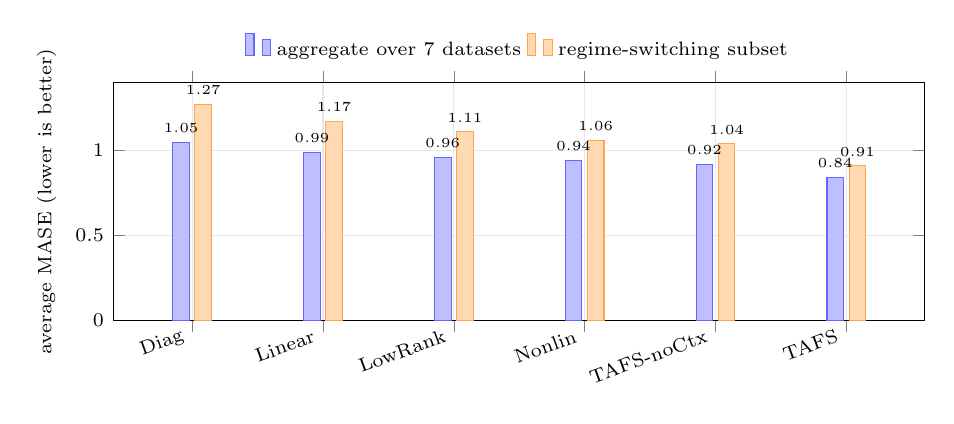
\begin{tikzpicture}
\begin{axis}[
    ybar,
    width=0.98\columnwidth,
    height=4.6cm,
    bar width=6pt,
    enlarge x limits=0.12,
    ymin=0.0, ymax=1.4,
    ylabel={average MASE (lower is better)},
    symbolic x coords={Diag, Linear, LowRank, Nonlin, TAFS-noCtx, TAFS},
    xtick=data,
    xticklabel style={font=\scriptsize, rotate=20, anchor=east},
    tick label style={font=\scriptsize},
    label style={font=\scriptsize},
    nodes near coords,
    nodes near coords style={font=\tiny, /pgf/number format/.cd, fixed, precision=2},
    grid=both,
    grid style={gray!18},
    legend style={font=\scriptsize, at={(0.5,1.05)}, anchor=south, legend columns=2, draw=none},
]
\addplot[fill=blue!25, draw=blue!60] coordinates {
(Diag, 1.05) (Linear, 0.99) (LowRank, 0.96) (Nonlin, 0.94) (TAFS-noCtx, 0.92) (TAFS, 0.84)
};
\addlegendentry{aggregate over 7 datasets}
\addplot[fill=orange!30, draw=orange!70] coordinates {
(Diag, 1.27) (Linear, 1.17) (LowRank, 1.11) (Nonlin, 1.06) (TAFS-noCtx, 1.04) (TAFS, 0.91)
};
\addlegendentry{regime-switching subset}
\end{axis}
\end{tikzpicture}
\caption{Central architectural ablation. Static feature transforms (diagonal, linear, low-rank, nonlinear) and a context-stripped variant (TAFS-noCtx) are compared against the full TAFS model on the aggregate of seven real datasets and on the regime-switching subset (Exchange + Istanbul Stock Exchange + Synthetic). The gap widens when the underlying regime is non-stationary.}
\label{fig:ablation_bars}
\end{figure}
